% Imported from topics/video-generation/seedance-2.5/integrated-design.md
\chapter{完整联合音视频候选架构}\label{seedance-m19}
\moduleinfo{M19}{候选设计与工程选型；组合效果待验证}{\hyperref[src-ltx-2]{\texttt{ltx-2}}、\hyperref[src-alchemint]{\texttt{alchemint}}、\hyperref[src-vace]{\texttt{vace}}、\hyperref[src-videocof]{\texttt{videocof}}、\hyperref[src-vincie-next]{\texttt{vincie-next}}、\hyperref[src-geometry-as-context]{\texttt{geometry-as-context}}、\hyperref[src-long-context-tuning]{\texttt{long-context-tuning}}、\hyperref[src-longlive]{\texttt{longlive}}、\hyperref[src-ltx-original-code]{\texttt{ltx-original-code}}、\hyperref[src-vace-code]{\texttt{vace-code}}、\hyperref[src-videocof-code]{\texttt{videocof-code}}、\hyperref[src-ltx-original-model]{\texttt{ltx-original-model}}}

至此各条输入和执行路径已有定义，下面将它们放回共同主干，检查完整候选系统是否相互兼容。

各模块已有了局部定义，现在把问题收回来：同一系统要读图片、视频、音频与结构条件，生成较长音视频，再定向修改，怎样形成一条可以训练的计算链？必须先选共同表示和主干，让时间、条件与目标在各处使用同样的含义。仅列出多篇方法的名称，还没有建立这种关系。

下面选定 LTX-2 初始公开系列的非蒸馏联合音视频模型作为共同主干，保留其 VAE、文本组件、双流 block 和原生 scheduler，再新增有绑定的参考记忆、源视频条件、区域定位与结构控制。它是面向类似公开能力的\textbf{完整候选设计}；尚未训练验证，也不代表 Seedance 2.5 的真实内部实现或同等效果。

\section{明确哪些保留，哪些新增}\label{seedance-m19-ux660eux786eux54eaux4e9bux4fddux7559ux54eaux4e9bux65b0ux589e}

{\def\LTcaptype{table} % do not increment counter
\small\setlength{\tabcolsep}{3pt}\renewcommand{\arraystretch}{1.18}
\begin{longtable}[]{@{}
  >{\raggedright\arraybackslash}p{(\linewidth - 4\tabcolsep) * \real{0.1900}}
  >{\raggedright\arraybackslash}p{(\linewidth - 4\tabcolsep) * \real{0.3900}}
  >{\raggedright\arraybackslash}p{(\linewidth - 4\tabcolsep) * \real{0.4200}}@{}}
\toprule\noalign{}
\begin{minipage}[b]{\linewidth}\raggedright
层级
\end{minipage} & \begin{minipage}[b]{\linewidth}\raggedright
选定设计
\end{minipage} & \begin{minipage}[b]{\linewidth}\raggedright
状态
\end{minipage} \\
\midrule\noalign{}
\endhead
\bottomrule\noalign{}
\endlastfoot
视频表示 & 原生视频 VAE，128通道，时间/8、空间/32 & 沿用共同基座 \\
音频表示 & 原生音频 VAE，约25个时间 token/秒、每时间位置128维 & 沿用共同基座 \\
文本 & 对应模型的冻结文本编码器、特征投影与连接器 & 必须匹配原系列 \\
生成主干 & 14B视频流＋5B音频流、原生跨模态交换 & 沿用联合建模方向 \\
参考记忆 & 独立素材编码、角色/类型/时间绑定、定额池化、门控读取 & 需要新增和训练 \\
源条件 & 待变/保留条件拆分、mask投影、残差 adapter & 需要新增和训练 \\
区域定位 & 自动区域预测或人工mask；可选编辑示例图 & 需要数据和新增任务 \\
空间控制 & 白模/depth/pose/camera条件与关键视角记忆 & 先实现已知结构路径 \\
长续写 & 从联合模型另派生因果块模型 & 单独训练，不是推理开关 \\
\end{longtable}
}

早期 Wan-1.3B 路线继续用于低成本阅读、机制和单能力实验；完整联合设计不把它的 latent 或权重接入 LTX。LTX 后续型号也不自动与这套原系列接口相同，实际工程以固定版本与模型配置配套。

共同基座具体选为原系列19B开发权重：48个联合块，视频宽4096、音频宽2048，split RoPE。新增模块位于第4、8直至48块之后，每处依次接源/结构残差、视觉参考和声音参考；参考支路内宽512，投影与门控逐处独立。完整维度、共享规则与参数保存方式见 \hyperref[seedance-m21]{模块契约}，不能仅凭原生构造器默认值替代实际权重配置。

\section{统一任务规格}\label{seedance-m19-ux7edfux4e00ux4efbux52a1ux89c4ux683c}

因此先把请求翻译成任务对象：时长、帧率、镜头计划、角色与 speaker、参考绑定、源视频、编辑范围、结构条件、音轨保持、种子和质量档位。后续每个模块都从这个对象取得自己的条件，不再独立猜一次用户要求。

\begin{verbatim}
用户要求
  → 任务编译与素材登记
  → 独立编码：文本 / 参考视觉 / 参考音频 / 源条件 / 结构
  → 按镜头和时间建立条件可见性
  → 联合视频与音频去噪
  → 解码、合法时长裁切、局部合成与音轨保持
  → 分项检查、定向返工或交付
\end{verbatim}

例如三十秒广告包含两个镜头：角色A前半段展示产品，后半段角色B加入；产品图只锁结构，动作视频只锁手部动作，声音参考只锁speaker A。若第二镜头的外套颜色错误，编辑请求保留角色、产品、动作和音轨，只重做指定区间的外套区域。

提示改写后，这些绑定仍要在。保留原始指令和编译结果，才能检查目标有没有被改变。一段更长的提示可以增加描述，却不能代替角色、素材和区间之间明确的对应。

条件还注明是用户给定、自动估计还是模型生成。自动区域低置信时先确认区域，主体冲突时先修绑定；结果若只错了某个镜头或局部，就沿该范围重做。身份、动作、台词、保持与返工最后按交付任务统计，而不是只留下最好的一次候选。

\section{共同潜空间与时间对齐}\label{seedance-m19-ux5171ux540cux6f5cux7a7aux95f4ux4e0eux65f6ux95f4ux5bf9ux9f50}

视频经原 VAE 得到：

\[
z_v\in\mathbb{R}^{B\times128\times T_v\times H_v\times W_v},
\quad T_v=1+(F-1)/8,\quad H_v=H/32,\ W_v=W/32.
\]

音频实现可保留 \codepath{B,8,Ta,16} 的 codec 布局，进入主干时每个时间位置整理为128维。音频约25个时间位置/秒；视频与音频仍通过物理时间而非索引一一对应。所有特征继承原模型归一化，不能为统一 shape 任意换 codec。

以三十秒、24fps为例，最终要720帧。为了满足 \(1+8k\) 的编码约束，可在模型内部使用721帧，输出裁为720帧，并保存补帧映射；音频严格保留三十秒。训练的padding有效位和像素监督不得把额外帧当成真实动作。latent边界覆盖多个像素帧，不能仅把最后一个latent粗暴置为无效。

\section{参考记忆的两条读取支路}\label{seedance-m19-ux53c2ux8003ux8bb0ux5fc6ux7684ux4e24ux6761ux8bfbux53d6ux652fux8def}

图片与视频进入视觉参考记忆，音频进入音频参考记忆，分别保存来源、主体、角色、时间、置信度与有效位。首版视觉预算2048、音频预算512；按每图32、每视频64、每音频32摘要token，30/10/10份素材在文件容量上可被表示，但质量必须逐级验证。

参考支路安插在每四个原生block后作为初始设计。先门控读取图像/外观与声音信息：

\[
\Delta h_v=g_v\operatorname{Attn}(Q_v,K_{r_v},V_{r_v};B_v),
\qquad
\Delta h_a=g_a\operatorname{Attn}(Q_a,K_{r_a},V_{r_a};B_a).
\]

新增支路先按镜头屏蔽不允许的主体，按时间加软偏置，并保留 null token。空间 query 本身没有 subject ID，只有已给布局、源跟踪或可靠预测区域时，才有依据作空间硬约束；其余绑定通过主体 embedding 与训练学习。两条流再经原生 AV 模块交换信息，声音也要遵守角色与 speaker 的映射，不能把归属全部留给 attention 去猜。

动作视频中的姿态、光流和相机走结构支路，需要时关闭原人物外观。音色克隆则用同 speaker 跨台词配对。于是“能输入声音”与“能保持指定音色”仍隔着相应的条件和监督，不能由接口存在推出能力已经学到。

需要保留对白或配乐时，完整干净音轨走对齐条件路径，不能压成32个音色摘要后期待逐字或逐拍一致。其时序token按原音频codec单独计费；多人同时说话时，混合音频token可能对应多个speaker，不能无条件强制一个token只绑定一个人。

\section{源条件与区域预测怎样接入}\label{seedance-m19-ux6e90ux6761ux4ef6ux4e0eux533aux57dfux9884ux6d4bux600eux6837ux63a5ux5165}

源视频再拆成待变、保留内容与 mask，分别对齐编码后进入 context adapter。带噪目标仍从原主干输入，新增支路在约定层加残差。参考图、源图和源视频独立编码，避免在 VAE 时间轴上制造本来不存在的连续关系。

用户没给 mask 时，先用 grounding、分割或训练得到的视觉区域预测定位；关键帧编辑对再提供原样到目标外观的对应。首版先把定位与生成分开，便于检查，不将源、区域与目标一开始全部堆进大序列。

这里干净源条件与目标覆盖又要分清。源条件不随目标去噪时间变化；目标的已知区若作重噪覆盖，则仍沿一条固定噪声路径变化。训练必须选明这种条件方式，否则同名输入在两处使用不同时间含义。

\section{原生双流块怎样保持同步}\label{seedance-m19-ux539fux751fux53ccux6d41ux5757ux600eux6837ux4fddux6301ux540cux6b65}

每个流保留自身self-attention、文本cross-attention、双向音视频cross-attention和FFN。流内视觉使用时空位置，跨模态Q/K只使用共同物理时间；对方的噪声状态通过调制与门控影响交换强度。

\begin{figure}
\centering
\pandocbounded{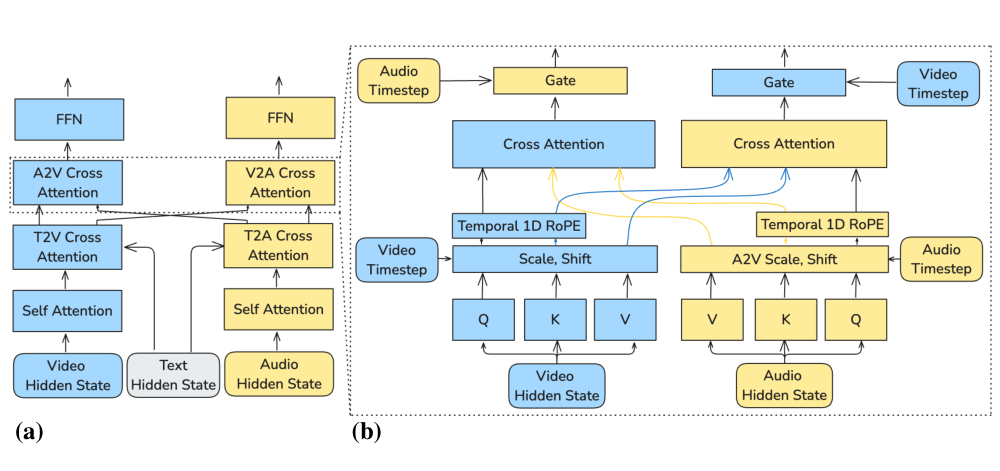
\includegraphics[keepaspectratio,alt={联合主干与音视频跨注意力的组成 （论文示意，来源：ltx-2）}]{assets/seedance/figures/joint-av-block.png}}
\caption{联合主干与音视频跨注意力的组成 （论文示意，来源：ltx-2）}
\end{figure}

交换时两边先读取同一组旧状态，再各自加残差。若先更新一边再给另一边读，执行顺序本身就改变了计算图。缺音轨时跳过无效目标和交互，真实静音仍监督；需要保留原音轨时，则把它作干净条件，输出复用，不为“联合”强行重生声音。

\section{一次采样的具体执行顺序}\label{seedance-m19-ux4e00ux6b21ux91c7ux6837ux7684ux5177ux4f53ux6267ux884cux987aux5e8f}

采样前可先缓存固定条件编码，再按任务决定哪些目标更新。可读条件、去噪更新、损失有效位和最终替换范围各有一个 mask：它们来自同一请求，但对应不同计算，因而分别保存。

{\def\LTcaptype{table} % do not increment counter
\small\setlength{\tabcolsep}{3pt}\renewcommand{\arraystretch}{1.18}
\begin{longtable}[]{@{}
  >{\raggedright\arraybackslash}p{(\linewidth - 6\tabcolsep) * \real{0.1600}}
  >{\raggedright\arraybackslash}p{(\linewidth - 6\tabcolsep) * \real{0.2800}}
  >{\raggedright\arraybackslash}p{(\linewidth - 6\tabcolsep) * \real{0.2800}}
  >{\raggedright\arraybackslash}p{(\linewidth - 6\tabcolsep) * \real{0.2800}}@{}}
\toprule\noalign{}
\begin{minipage}[b]{\linewidth}\raggedright
任务
\end{minipage} & \begin{minipage}[b]{\linewidth}\raggedright
视频状态
\end{minipage} & \begin{minipage}[b]{\linewidth}\raggedright
音频状态
\end{minipage} & \begin{minipage}[b]{\linewidth}\raggedright
模型更新与交付
\end{minipage} \\
\midrule\noalign{}
\endhead
\bottomrule\noalign{}
\endlastfoot
文本/参考生成音视频 & 带噪目标 & 带噪目标 & 联合更新与解码 \\
仅有视频监督 & 带噪目标 & 缺失标记 & 只更新视频，屏蔽无效AV连接 \\
保留源音轨的视觉编辑 & 带噪目标＋干净源视觉条件 & 干净源音频条件 & 只更新视频，交付复用原音轨 \\
因果续写 & 干净历史＋当前带噪块 & 干净历史＋当前带噪块 & 仅更新当前块，两流遵守相同历史边界 \\
\end{longtable}
}

保留音轨与缺音轨是新增任务策略，训练必须出现相同状态，不能只在推理时把音频噪声改成零。干净音频仍可提供口型条件，缺音轨则完全不提供有效声音信息。

还需把模态存在、隐藏计算和 latent 更新分开。保留声音时，输入音频 latent 固定且干净，不计算音频 loss，也不更新它；声音流仍参与 AV 计算。其深层状态一旦读取当步视频，就仍随步数变化，所以默认只缓存 codec 结果，Transformer 声音特征每步重算。

\begin{verbatim}
1. 编译任务，确定内部帧数、补帧映射、两流时间坐标和各类mask。
2. 独立编码参考、源内容和结构；按模型/内容/变换版本缓存。
3. 未给区域时先定位；确定区域后编码待变/保留条件。
4. 活动目标从噪声起步，沿版本固定的sigma序列调用联合主干和新增支路。
5. 每步只更新活动目标；可选已知区重噪覆盖使用同一固定噪声路径。
6. 解码并按媒体时钟裁切；源像素与源音轨按交付规则直接合成。
7. 检查目标变化、外区保持、声画同步和角色状态，定向返回失败步骤。
\end{verbatim}

新增参考strength首先作为门控残差的缩放量，独立于原生guidance保存。短片保留原生采样配置作对照，长片候选采用有界长度shift并与训练噪声课程配套；这是需要比较的新选择，见 \hyperref[seedance-m25]{数据与训练规格}。具体步数从配套配置读取；尚未进行少步数训练时，不指定一个未经验证的高速档位。

\seedancenetworkfigure{5}{Seedance 2.5 推测方案的联合采样回路与两种长视频执行关系。图中主干沿用总览章的 Dual-MMDiT 推测；本章 LTX 替代实现说明同类执行接口，不表示二者逐层拓扑相同。}{fig:seedance-joint-inference}

\section{联合长片与因果续写分别保存版本}\label{seedance-m19-ux8054ux5408ux957fux7247ux4e0eux56e0ux679cux7eedux5199ux5206ux522bux4fddux5b58ux7248ux672c}

第一版先保留整段联合去噪，按 8、16、30 秒任务逐步训练，全局连接作质量对照。因为视频和声音状态每步都变，这一版不使用跨步历史 KV 来声称精确复用。先看长程条件是否真的保持，再改依赖结构。

续写模型从它另行派生：以约4秒的时间块为单位，块内双向，块间只能读历史；视频和音频都采用同一块时间边界，四类流内与跨模态注意力都不能偷读未来。编码依赖越过边界的token延迟入块。训练先以真实/扰动历史起步，自生成历史需由teacher按实际历史重标后续并过滤状态冲突，历史梯度截断。

缓存的是在固定提示/参考/坐标/零噪声历史条件下生成的层状态。每块采样结束后须按干净历史重算再写入，不能提交最后一个带噪步的K/V。每次提示或过去内容改变，对相应依赖全量重建为正确性基线。原decoder并非无前瞻流式设计，首版整段解码交付；完整协议见 \hyperref[seedance-m24]{长视频执行规格}。训练未完成前，可用尾段重叠条件做续写，但应如实记为``条件续写''，不能宣称已获得实时AR缓存能力。

\section{白模与长程空间记忆}\label{seedance-m19-ux767dux6a21ux4e0eux957fux7a0bux7a7aux95f4ux8bb0ux5fc6}

已知白模先渲染同步depth/normal/pose/camera射线，经过type专用投影与context adapter进入视频流。静态结构、动态主体状态、带置信度的关键视角分开保存，每镜头检索少量可见且相关的历史视图。

首版不要求同时恢复完整世界，生成图像的深度也不作为精确几何真值。已知 CAD 给定的约束与后续学习型几何预测，来源和确定程度不同，应分别监督。

\section{三十秒的成本必须先算清楚}\label{seedance-m19-ux4e09ux5341ux79d2ux7684ux6210ux672cux5fc5ux987bux5148ux7b97ux6e05ux695a}

取内部721帧、\(512\times896\)分辨率，无额外空间patch时：

\[
N_v=91\times16\times28=40\,768,\qquad N_a\approx750.
\]

视频dense attention每头约有16.6亿个连接；单方向音视频交互约3060万个；2048视觉参考的完整交叉读取约8350万个。Flash attention避免显式保存完整矩阵，却不会消除算术量。

这也解释了从短片、小分辨率和少量参考开始的原因。扩到 30 秒后，显存分片、context parallel、条件预算与训练课程都要跟上。窗口、稀疏和少步数可再优化，但需要质量对照，不能预先作为无损能力计入。

\section{方案的完成边界}\label{seedance-m19-ux65b9ux6848ux7684ux5b8cux6210ux8fb9ux754c}

到这里，共同主干、表示、条件路径、训练任务，以及两种长视频方式，已经有了对应关系，可以逐块实施。仍待实验回答的是：压缩参考后细节是否足够，复杂动作能否稳定到三十秒，音色与局部保持能否达到要求，以及训练要花多少资源。这些不能由结构图本身推出。

真实联合音视频与训练从 \href{https://github.com/Lightricks/LTX-2}{LTX-2} 进入；统一视觉条件借鉴 \href{https://github.com/ali-vilab/VACE}{VACE}，区域定位式编辑看 \href{https://github.com/knightyxp/VideoCoF}{VideoCoF}，因果流式机制看 \href{https://github.com/NVlabs/LongLive}{LongLive}。迁移这些机制仍是新增工作，不是现成仓库之间的一键连接。

可逐项审阅的 \href{https://github.com/foocker/multimodal-journey/blob/0f1b6bb86d609d75d8c2582063d85707d0180d39/topics/video-generation/seedance-2.5/design-spec.json}{设计规格} 保存形状、预算、依赖与训练候选值；已固定checkpoint的revision、文件名和远端声明哈希，并读取配置与文件头，张量载荷尚未下载，本地完整校验哈希为空。完整训练课程另见 \hyperref[seedance-m20]{联合训练配方}，资源与返工口径见 \hyperref[seedance-m26]{推理与交付规格}。
